\chapter{Conclusion}

% Example: find photograph that is used in multiple stories. Place in context of

Stories are increasingly becoming multifarious media texts, consisting of numerous interlinking fibers that each constitute different narratives of their own. Some of these texts are traditional --- photographs, audio, video, maps, charts, and graphs --- while others are something a bit new, emerging as a combination of these media. Journalism has always relied on data, but data can now flow with the narrative arc of a story in new ways. Interactive pieces, special features, and standalone applications often expand the rules of the hyperlink and bypass the URL, taking advantage of the new capabilities of HTML5 and modern JavaScript frameworks. As stories increasingly become networked and interactive, they explode into something more like apps.

An app can take many forms: it can live on the Apple or Google app store, whether for a phone or a tablet (known to developers as a ``native'' app); or an app can simply be a web product that is a bit \emph{more} than a static webpage, or a single story. Its information might update on the fly, or it might feature advanced interactive elements inspired by documentary film and gaming; some of these take advantage of traditional hypertextuality, but others rely on hovering, swiping, watching, and listening rather than clicking and reading. There is a sort of continuum between traditional narrative stories and interactive applications, and most emerge as a sort of hybrid. The New York Times' Pulitzer-winning 2012 piece ``Snow Fall'' is the most canonical example of such a mixture of story and application.\autocite{branch_snow_2012} These stories stretch the traditional link- and URL-based navigational scheme of the web to its limits. Native apps go even farther than interactive stories, sometimes offering views and glimpses of the web (for instance, think of clicking on a link in your Facebook or Twitter app and being led to a webpage), but excluding search or URL-based navigation from the experience.

Modern publishing platforms, such as Medium or Storify, can serve as factories for expanded news stories, which blur the divide between content and context and begin to veer into app territory. Such platforms allow writers to incorporate a variety of media, and take as a given that online stories combine original creation with remix and curation. Tools that facilitate annotation, such as Genius, further complicate the picture, tying texts to links, tags, and other commentary. Here stories are treated as systems from the outset, consisting of a plethora of media types. There is no doubt that modern web browsers and applications offer compelling new user experiences, and some parts of the web have essentially outgrown their need for traditional links. The link has limitations of its own, after all, which I explored at length in Section 2.3. But in terms of archiving, storage, and face-value navigation, URLs and links are often all we have to go by; the URL, after all, serves as the default archival unit for the Internet Archive. While dynamically-generated web pages have been around since the early days of the web, recent years have seen an increasing reliance on browser-side scripts to generate webpages; this approach offers far greater flexibility in presentation and user experience, but it limits its historical potential, reducing the page's data and structure to the technologically contingent lines of code that generate it. Modern JavaScript not only bypasses the link's function, but often runs explicitly counter to it; the anchor tag is sometimes repurposed for customized use, and JavaScript's commonly-used \texttt{preventDefault} function actively stops the link from performing its usual task (that is, jumping you to another part of the web).

In this conclusion, I will consider the expanding future of the hyperlink. How is the traditional, default, cornerstone ``jumping'' action of the web --- so crucial to the web's size, shape, and political economy --- being bypassed or made obsolete in the next generation of stories? How are theorists, designers, and platforms alike rethinking the nature of the link, and therefore the roles of attribution and citation? Finally, how is the resulting change affecting the user's experience of the web, and its future archivability? I will begin with a typology of what I consider ``news apps,'' and the challenges with preserving the process and results behind them. I will then look to certain designers' reconceptualizations of the hyperlink, and their potentials for alternative use; here I will also consider linking within mixed media such as audio and video, afforded by HTML5. Finally, I will conclude by considering artistic treatments and considerations of archives, which offer a window into a user's experience of the link amidst this information deluge.

% Anne Helmreich and that other guy...

\section{From links to apps}

Some newsrooms are beginning to form dedicated internal teams for the production of interactive applications. Public, private, and nonprofit media alike are creating ``news apps teams'' that straddle the line between journalism and software development. A 2014 panel at the Online News Association, co-led by the Wall Street Journal and the Texas Tribune, closely considered how to build such a team in a newsroom, and similar outfits can be found at the Chicago Tribune, ProPublica, NPR and the Guardian.\autocite{mcbride_how_2014} Featuring journalists who are equally comfortable writing in English and JavaScript, or calling sources and wrangling datasets, these desks signal a new future where editorial and tech are fully integrated and managed by multitalented generalists.

Given the increasing proliferation of context, multimedia, and interactivity built into today's stories, this turn towards apps seems a logical next step. News apps aim to blend the bundle of story and information, by creating bespoke platforms and containers that serve to perfectly complement the right story with the right navigation and presentation. Sometimes these applications are even built outside of the content management system of the organization; while the CMS is a factory for stories, it cannot always contain apps. Apps come in a variety of shapes and sizes, and each brings its own challenges for standardization, organization, archivality and reuse. This makes summarizing their future and associated challenges difficult; here I will aim to define a sort of typology of apps and platforms that challenge or expand the hyperlink's basic function, through the lens of the difficulties around archiving such works.

First, news apps come in the form of aggregation, personalization, and recommendation tools. These often take the form of native mobile apps, and have usually been the purview of information technology companies; some examples include Flipboard, Prismatic, and LinkedIn's Pulse. As publishers begin increasingly aggregating and linking out, though, there is a new potential niche for such products tied to newsrooms. BuzzFeed's news app features stories from around the web, as ``part of a collaborative project with other news outlets.''\autocite{odonovan_buzzfeed_2014} While it is a publisher's product, the app is taking cues from aggregators like Yahoo! News Digest and Circa for design and recommendation decisions; similar efforts are coming from the New York Times, whose NYT Now app and front-page ``Watching'' section both reflect a desire to link out more often. Moreover, while these publishers have long focused on the importance and role of social media in their business, they are increasingly creating content directly for outlets like Facebook and Snapchat.\autocite{isaac_facebook_2015} These social ranking and recommendation tools seem to promote open linking across different parts of the web, but just as often they may encourage continuous scrolling, browsing, and watching rather than clicking and reading.

A second type of news app to consider are standalone sites, usually data-driven and self-updating, that offer compelling statistics and narratives with design playing a crucial role. Often these state a specific role of adding context and explanation to a story. Sometimes these are not affiliated with any mainstream legacy publisher, such as Laura and Chris Amico's Homicidewatch.org, which combines stories and data to track every homicide in certain major urban areas. New York-based News Deeply aims to create platforms that enhance the user experience of news as well, combining statistics, maps, and timelines to tell a larger narrative instead of a single story; early experiments have tracked the Ebola pandemic and the Syrian civil war. Perhaps the most telling example is Timeline, a mobile app whose tagline succinctly summarizes the contemporary turn towards context: ``The news is the short tail of a very long string of events. \emph{Timeline} weaves those events into rich, compelling stories.''\autocite{_timeline_????} These apps and standalone sites are evolving repositories of code in their own right, and they call into question the dominant role of stories, and the content management systems that generate them.

The final type of news app that challenges the conventions of hyperlinking is the multimedia storytelling platform. Applications like Medium, Storify, and MIT Center for Civic Media's FOLD fall under this rubric. Like most content management systems, these applications still produce stories; but their notion of what a news story \emph{is} is reflected in the types of media that can be collected and embedded within them. These platforms provide a system for easily incorporating tweets, videos, maps, and graphs. While they treat the story as a multithreaded media text and push the boundaries of the story in greater or lesser degrees, they still follow certain conventions and rules; in FOLD's case, for instance, the text proceeds vertically, while contextual multimedia elements are presented horizontally to offset it. This results in a balance between convention and innovation in storytelling; such systems offer the promise of allowing new forms of expression without breaking or challenging archival standards.

In each of these cases, and as news increasingly adopts elements of documentary film and gaming, the language and formats of storytelling are changing. This leads to particular challenges in storage and archiving. In one sense, these apps form a symbiotic relationship with archives; an application like Timeline aims to keep archives alive and dynamic in the context of today's stories, while data-oriented apps tend to be built with information sustainability in mind. All the same, their many forms lead to difficulty in standardized storage. Scott Klein, luminary of news apps at the \emph{New York Times}, brings up Adrian Holovaty's ChicagoCrime.org, which Holovaty described as ``one of the original map mashups.''\autocite{holovaty_memory_2008} Launched in 2005, it is now defunct and unreachable in its original form; while the data survives, we have lost the presentation, and more importantly, the work, process, and context behind it.

There is no doubt that some apps must be retired when their event passes or their function is completed. Software constantly races against obsolescence, and code is an ephemeral and evolving artifact. With some level of forethought, apps can be saved, stored, and archived; but what is important and worth saving about a given application? Is it the visual design, the data, or even the process of building it? In March 2014, a group of attendees of the NICAR conference gathered at Washington, D.C.'s Newseum to brainstorm the challenges and potentials of preserving news apps, suggesting more collaboration with libraries, museums, and cultural heritage institutions.\autocite{_opennews/hackdays/archive_????} The Library of Congress has pledged to aid in digital preservation of newspapers, and some institutions are offering novel ways of preserving and maintaining digital work for the future. At the Cooper Hewitt Smithsonian Design Museum, a team led by Sebastian Chan has been preserving a defunct Silicon Valley app called Planetary as ``a living object.'' For the Cooper Hewitt, preserving an app is more like running a zoo than a museum: ``open sourcing the code is akin to a panda breeding program.''\autocite{chan_planetary:_2013} They'll preserve the original, but also shepherd the open-source continuation of app development, thereby protecting its offspring and suggesting new applications for old frameworks. While the Cooper Hewitt is currently guarding Silicon Valley technology, overlaps and partnerships between newspapers and cultural heritage institutions could lead to similar experiments.

These data-driven apps demand a great deal of work at the outset, which makes them high-investment projects for publishers, with high return expected as a result. This means that the most high-profile, engaging interactives tend to pair with ``slow news'' or predictable events with guaranteed audience, such as the World Cup or the Oscars. Unless such platforms become increasingly standardized, it will be difficult to produce data-driven and interactive stories about breaking and unpredictable events. What are the implications of this for archivality, storage, and history? How can we balance the creative adventurousness of new forms of storytelling with a particular set of frameworks and standards that will allow them to be legible to the public, and archivable for history?

News sites are, after all, increasingly linked to one another, and saving a single page out of the internet is itself an exercise in futility. The work of the members of the Amsterdam-based Digital Methods Initiative especially brings home this point; Anne Helmond's research into the Internet Archive examines the ``boundaries of a website,'' exploring where content ends and context begins. She finds, echoing Niels Br\"{u}gger's work into web archives, that pages (content) are privileged over sociotechnical context. Richard Rogers' \emph{Digial Methods} laments the inability of current digital archiving methods to highlight ``the references contained therein (hyperlinks), the systems that delivered them (engines), the ecology in which they may or may not thrive (the sphere) and the related pages, profiles and status updates on platforms.''\autocites{helmond_exploring_2013}{rogers_digital_2013} Helmond then examines the phantom, broken links to dozens of advertising and analytics platforms on a typical archived New York Times page. The Open Knowledge Foundation approaches the same phenomenon from an online privacy angle; in their 2014 project ``The News Reads Us,'' they find that German news outlets like \emph{Die Welt} generate links to up to 60 other websites under the hood, with much of their data feeding straight to analytics platforms at Google and Facebook.\autocite{wehrmeyer_news_????} Here we see a small-scale example of the larger information flows suggested by the source-authority-hub model in section 4.1.2. Thus content is not the only information consistently flowing from publishers to platforms; user data also gets aggregated in turn.

\section{Standardizing stories}

The online publishing platforms of today still tend to read linearly, but special features and apps are beginning to expand stories into two dimensions. The linear feed or stream is the simplest to understand, but limits storytelling capabilities and audience literacy as a result. Users tend to read digital stories in two dimensions: the X-axis is for browsing, while the Y-axis can be better used for deep dives. A platform like FOLD reflects this standard, with linear cards supplemented by context along the Y-axis. FOLD therefore imposes certain creative limitations, giving a storyteller more linking potential than a single webpage, but less than an entire website. This not only allows for easier development and reuse, it lets audience literacy to develop over time, and creative exploration of the form. FOLD will soon have the ability to embed other FOLD cards, allowing for links between stories themselves. FOLD is a sort of factory for a certain type of linked story, a content management system on a higher plane. Best of all, it allows storytellers a different dimension of expression with little to no technical effort; while ``Snow Fall'' was rightly lauded, Quartz's Kevin Delaney quipped ``I'd rather have a Snow Fall builder than a Snow Fall.''\autocite[36]{_innovation_2014} Rather than continuously building apps and special features, some publishers are striving to turn their CMS into a factory for rich interactives as well as simple stories.

\begin{figure}[ht]
\centering
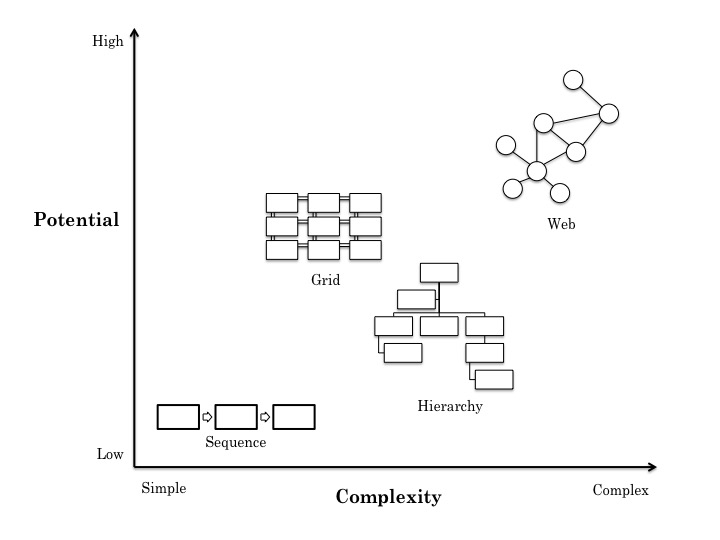
\includegraphics[width=6.0in]{figures/linkstructures-custom}
\caption{Diagram of some standard link structures. Adapted from Blustein 1999.}
\label{fig:linkstructures-custom}
\end{figure}

Other standards are also changing the web and its narratives in enticing new ways. HTML5 was completed in October 2014, the first official update to the web in decades. It brings with it powerful features across a range of devices. Some of these aim to enrich the semantic meaning of content, with new standardized tags like \texttt{<section>} and \texttt{<article>}; others bring hypertext to other rich media, such as \texttt{<audio>}, \texttt{<video>}, and \texttt{<canvas>}. All of these tags allow for richer forms of automatic navigation and data collection, giving multimedia some of the jumping and contextualizing powers of the hyperlink. Some also offer new forms of linking; with HTML5, sound and image elements can themselves be made interactive, and a lot of them adopt the mechanics of the link and the rich semantic backup of hypertext.

Consider, for instance, the \texttt{<audio>} tag, which by default places an audio player on a page. Previously, audio required a plugin (such as Adobe's Flash), and did not adhere to any standards; now, audio files can contain associated text, variable play modes, and detailed time and playback information. This not only improves the user experience and enables new modes of presentation for developers, but it also lets audio be more searchable and discoverable online. For example, a radio interview about climate change is no longer a meaningless block of audio to a web browser; if a user were only interested in the sections about solar power, or wanted to hear all of the questions but not the answers, HTML5 might enable the user to ``jump'' to different sections of the audio. San Francisco-based startup Pop Up Archive automatically transcribes spoken word audio, aiming to provide precisely the sort of discoverability and research assistance through audio that both expands on and bypasses hypertext.

As we have seen, the story does not end with the story itself, and the myriad contextual elements---from auxiliary photos, to charts and graphs, to ads and popups---are as much part of the experience of online journalism as the text itself. Yet another layer is added to the archive through the social metadata that travels with a given story, as well; when a reader registers a comment, click, or like on a story, this too is archived along with it. Recent years have seen a focus on digital annotations, or comments that are tied to specific sub-pieces of text rather than comments that appear at the bottom of a page. The goal of multimillion dollar company Genius is to ``annotate the world,'' while more scholarly startup Hypothes.is asks you to ``annotate with anyone, anywhere'' (and a promotional video on their homepage prominently features Vannevar Bush's memex). Publishers like Atlantic Media's Quartz and platforms like Medium are also incorporating side-by-side annotations, rather than end-of-page comments. This approach privileges commentary, placing it on a similar level to the original content.

The W3C --- the web's standards organization --- is developing a series of standards for annotation, which will allow for multimedia, as well as annotations \emph{of} annotations. This again points to the recursive nature of knowledge, and a need for similar structures when archiving and storing it. It also emphasizes the inherent challenges in providing concrete commentary on ephemeral content; many of its technical challenges --- such as what to do with an annotation if the source text is deleted --- allude to deeper and more philosophical challenges inherent in the web itself. The effort to standardize annotation also reflects the primacy afforded to online commentary---more often found on social media platforms than end-of-page comment sections---and a need to consider these socially contextual elements as a potential part of the archived story as well.

\subsection{Future design}

Some designers and institutions are also reconsidering the look and feel of the hyperlink. These approaches assume that this basic jumping mechanic is not going away anytime soon, so the trick is to give it better interactive capabilities and differential nuance. Australian researcher and founder of NewsCubed, Skye Doherty, has especially considered these limitations of the link, also noticing parallel limitations in the treatment of hyperlinks by researchers. While online link analysis considers the location and direction of links, and qualitative reviews address the use of links by information gatherers and providers, there is little research that combines these broad treatments with user experience and narrative structure.

Indeed, hypertext found perhaps its first ally in fiction and art; scholars like George Landow, Jay David Bolter, and Lev Manovich have traced the use of hypertext as a narrative device that champions a proliferation of narrative and collapses linear forms of storytelling. Early experimenters in hypertext were often not information technologists, but writers and artists looking for new forms of expression that integrated image, text, and sound.

These digital literary scholars have focused on hypertext's artistic and literary potential, and often highlighted pre-echoes of nonlinear writing that hypertext brings to the fore, especially in modernist literature. The ``inter-cutting'' techniques that eschew chronological and single-voiced narrative found in works like James Joyce's \emph{Ulysses} and Virginia Woolf's \emph{The Waves} point to the limitations of language and an inspiration from narrative techniques that were new at the time, borrowing from film, radio, and the clipped, decontextualized print of newspapers. In these cases too, writers and thinkers like Joyce and Walter Benjamin saw the creative value of obsessive collection and curation. Justin Hall, one of the web's first popular ``weblog'' writers, wrote in 1993 that his blog stemmed from ``A deep geek archivist's urge to experiment with documenting and archiving personal media and experience. In college I realized that Proust and Joyce would have loved the web, and they likely would have tried a similar experiment---they wrote in hypertext, about human lives.''\autocite{gillmor_we_2006}

Since hypertext's early pioneers were writers and artists experimenting with a new form, it is surprising to see this body of work and research ignored in favor of quantitative link analyses, whether beginning from network science or social science. This is not to say that such analyses are not useful, but that they are only part of the picture; Doherty asserts that hypertext ``is under-researched in journalism practice, particularly as a narrative device.''\autocite[124]{doherty_hypertext_2014} As journalism continues to balance warily on the fence between ``stories'' and ``information,'' analyses of journalism and hyperlinks could combine these divergent research paths, both understanding hypertext's effect on narrative structure on a small scale, and its foundational role in contextual network formation at a larger scale. In order to bring in new design and storytelling potentials to hypertext scholarship, journalism can serve as a crucial bridge between big data and small story.

Much of the utopian rhetoric around the web has fallen away in recent years, perhaps replaced by similar discussion around big data. Early-web writings on hypertext by Manovich, Bolter, Landow, and others sometimes treated the hyperlink as a tool of liberating power and narrative freedom, but this rhetoric has since been tempered by its role as a device for tracking and directing user behavior. Doherty's aim is to bring back the early web spirit of the hyperlink's potential, and expand it into the contemporary web. In considering new models and interactions for the hyperlink, Doherty emphasizes its spatiality, which I address historically in section 3.2.2. He notes that few modern tools offer graphical maps of a document's or website's structure, despite that some such views used to play ``an important role in authoring (and also navigating) hypertext.''\autocite{doherty_hypertext_2013} Journalism literature does not consider how ``hypertext exists in space.''\autocite{doherty_hypertext_2013} Spatial, dimensional expressions of hypertext can help users and writers alike see the overarching structure of a story. Stories can take on a variety of graphical structures, some of which can be standardized, while others expand or break a typical model of story complexity. The applications, features, and factories for new stories are breaking the traditional notion of the hyperlink as a blue, underlined string of text, and playing to the strengths of the web as never before; Larrondo Ureta suggests that online special features exhibit ``one of the maximum expressions of hypertextuality.''\autocite{doherty_hypertext_2014,ureta_potential_2011} The challenge lies in maintaining this creative potential while still standardizing them enough to visualize, coherently read, and archive them.

Doherty concludes by proposing three models of ongoing stories in journalism, which offer two competing narrative approaches. The ``martini glass'' emphasizes author-driven narratives, while the ``drill-down story'' prioritizes a reader-driven approach. A third type, the interactive slideshow, promotes a dialogue between the two approaches, balancing author control and user navigation. While this typology is surely too-simple and does not account for the rich possible narrative, it points to a desire to begin to standardize and develop a language around interactive features, which break current boundaries and therefore current methods of storage, archivality, and reuse.

\section{The art of the archive}

The artist Lara Baladi does not want people to forget about Tahrir Square and \#Jan25. Although it was ``the most digitally documented and disseminated event in modern history,'' the 2011 Egyptian revolution is slipping into the past, and Baladi has gathered and stored thousands of media artifacts surrounding it.\autocite{baladi_vox_????} Her resulting project, \emph{Vox Populi: Archiving a Revolution in the Digital Age}, combines the latest news and ancient history, featuring documents ranging from a printout of the Declaration of the Rights of Man to a dynamic visualization of Twitter activity at the moment that president Hosni Mubarak resigned. In 2014, as a  I attended an early study for Baladi's project at Harvard's Graduate School of Design. Baladi had taken over a room and assembled an overwhelming array of media artifacts, surrounding the participants with such a variety of formats that sensemaking seemed impossible. But soon patterns started to emerge. The event featured tea and popcorn, while photos of popcorn machines at Tahrir Square gave a sense that we were experiencing the smells of the protest. Hard-copy printouts of Twitter conversations mixed with ancient artifacts projected onto TV screens, mimicking the mix of ancient and modern, and of digital and physical. This blend reflected the simultaneous revolutionary activity on the streets and online. These many representations combined with my own memory of reading about the protests from afar, and many of the artifacts on display intentionally reminded me that this was only a sliver of the real thing.

Baladi invited us to sit in a circle, drinking tea and discussing how the exhibit around us made us rethink the flow of history and its digital representations. As we talked, we were being constantly documented ourselves; photographers and videographers surrounded us snapping pictures and videos. Our discussion of the archive was being folded back into it. The urgent news of the seventeen-day revolution is sliding towards history, but Baladi's act of archiving it is far from an exercise in cold storage. By talking about the archive, we became part of it, reanimating the past and the people and ideas behind the Egyption revolution. \emph{Vox Populi} conjures up the exuberance and the fear at Tahrir Square in 2011, the ``unstuck-in-time'' qualities of social media, the age-old drive to collect and remember, and the tragic irony of struggling to hold onto memory in the age of information. As all of these traces remind us, we had to be there---but at least we have all of these traces.
%Any act of archiving, like any act of journalism, serves to influence the profile of its target, affecting our memory of it, and our associations with it. 

% Skye Doherty, Santa Cruz person

% Annotation

% APIs
